\documentclass[addpoints]{exam}

\usepackage{amsmath}
\usepackage{amssymb}
\usepackage{graphicx}
\usepackage{hyperref}
\usepackage{multicol}
\usepackage{tikz}
\usepackage{titling}

% Header and footer.
\pagestyle{headandfoot}
\runningheadrule
\runningfootrule
\runningheader{CS 113 Spring 201}{HW 3: Inference and Relations}{\theauthor}
\runningfooter{}{Page \thepage\ of \numpages}{}
\firstpageheader{}{}{}

\boxedpoints
\printanswers

\newcommand\union\cup
\newcommand\interx\cap

\graphicspath{{images/}}

\title{Homework 3: Inference and Relations}
\author{associative-multiset}  % replace with your team name
\date{CS/MATH 113 Discrete Mathematics\\Habib University, Spring 2022}

\begin{document}
\maketitle

\begin{questions}

  \section{Inference}
  
\question Prove the following arguments using inference rules. Mention the rule(s) that you use at each step.
  \begin{parts}
    
  \part[5] $ $\\
    \begin{tabular}{ll}
      P1 &  If it is Sunday today, then we play cricket or basketball.\\
      P2 &  If the basketball field is occupied, we don't play basketball.\\
      P3 &  It is Sunday today, and the basketball field is occupied.    \\
      \hline
      C & We play cricket or volleyball. 
    \end{tabular}
    \begin{solution}\\
      % Write your solution here
      P = It is Sunday today.\\
      Q = We play cricket.\\
      R = We play basketball.\\
      S = Basketball field is occupied.\\
      T = We play volleyball.\\
      \textbf{Premises:}\\
      $P1 = P \rightarrow Q \vee R$\\
      $P2 = S \rightarrow \neg R$\\
      $P3 = P , S$\\
      $C = Q \vee T$\\
      \textbf{Proof:}\\
      \[
        \begin{array}{c|c|c}
          Equation No. & Operation              & Rule                             \\
          \hline
          i            & P \rightarrow Q \vee R & Premise (P1)                     \\
          ii           & P                      & Premise (P3)                     \\
          iii          & R \vee Q               & Modus Ponens (i),(ii)            \\
          iv           & S \rightarrow \neg R   & Premise (P2)                     \\
          v            & S                      & Premise (P4)                     \\
          vi           & \neg R                 & Modus Ponens (iv),(v)            \\
          vii          & Q                      & Disjunctive Syllogism (iii),(vi) \\
          viii         & Q \vee T               & Addition (vii)                   \\
        \end{array}
      \]
    \end{solution}
    
  \part[10]  $ $\\
    \begin{tabular}{ll}
      P1 &  Ahmed failed the course, but attended every lecture. \\
      P2 &  Everyone who did the homework every week passed the course. \\
      P3 &  If a student passed the course, then they did some of the homework.\\
      \hline
      C & Not every student did every homework assignment.
    \end{tabular}

    \begin{solution}\\
      % Write your solution here
      Assuming the following domain\\
      $s$ = Students enrolled in the course.\\
      $w$ = Weeks of thhe semester.\\
      Translating the above premises into logic.\\
      P1 = $\neg P(b) \wedge \forall w(L(b,w))$\\
      P2 = $\forall s[(\forall w H(s,w)) \rightarrow P(s)]$\\
      P3 = $\forall s [P(s) \rightarrow \exists w H(s,w)]$\\
      C = $\exists s \exists w \neg H(s,w)$\\

      \textbf{Proof:}\\
      \[
        \begin{array}{c|c|c}
          Equation No. & Operation                                      & Rule                            \\
          \hline
          i            & \neg P(b) \wedge \forall w(L(b,w))             & Premise (P1)                    \\
          ii           & \neg P(b)                                      & Simplification (i)              \\
          iii          & \forall s[(\forall w H(s,w)) \rightarrow P(s)] & Premise (P2)                    \\
          iv           & \forall w H(b,w) \rightarrow P(b)              & Universal Instantiation (iii)   \\
          v            & \neg \forall w H(b,w)                          & Modus Tollens (iv),(ii)         \\
          vi           & \exists w \neg H(b,w)                          & QuantifierNegation (v)          \\
          vii          & \exists s \exists w \neg H(s,w)                & Existential Generalization (vi) \\
        \end{array}
      \]
    \end{solution}
  \end{parts}

\question[5]
  Consider the statement: The remainder of the square of any odd number when divided by 4 is 1.
  
  \begin{parts}
  \part[5] Write the above statement using predicate logic notation and prove it.
    \begin{solution} \\
      % Write your solution here
      Domain: $\mathbb{Z}$\\
      O(x): x is an odd number\\
      R(x,d,r): remainder of x when divided by r\\
      Then, $$\forall x O(x) \implies R(x^2,4,1)$$
      The predicate can be written mathematically as follows: 
      $$\forall x \exists k : x = 2k + 1 \implies \exists m x^2 = 4m + 1$$
      Let the premise be true, then:
      \begin{gather*}
        x = 2k + 1\\
        \implies x^2 = (2k + 1)^2\\
        = 4k^2 + 4k + 1\\
        = 4(k^2 + k) + 1\\
        = 4m + 1 \text{       where, } m = k^2 + k
      \end{gather*}
      Hence proved.

    \end{solution}
    
  \part[5] Write the statement from above using a bi-conditional instead of a conditional. Prove whether the new statement holds.
    \begin{solution}\\
      % Write your solution here
      The bi-conditional statement would be as follows:
      $$\forall x O(x) \iff R(x^2,4,1)$$
      Since, the forward implication has already been proved, therefore we now need to prove the backward implication, i.e.
      $$\forall x  R(x^2,4,1) \implies O(x) $$
      Using proof by contraposition then,
      $$\forall x \neg O(x) \implies \neg R(x^2,4,1)$$
      $$\forall x E(x) \implies \neg R(x^2,4,1)$$
      Let the premise be true, then:
      \begin{gather*}
        x = 2k\\
        x^2 = (2k)^2\\
        = 4k^2\\
        = 4m \text{       where, } m = k^2\\
        \implies R(x,4,0)
      \end{gather*}
      Hence proved.
    \end{solution}
  \end{parts}

\question[5]
  Show that these statements about the real number $x$ are equivalent: (i) x is irrational, (ii)  $\frac{x}{2}$ is irrational. Which proof method did you use?

  \begin{solution}\\
    % Write your solution here
    Two statements (i) and (ii) are equivalent, if (i) $\rightarrow$ (ii) is true and (ii) $\rightarrow$ (i) is true.\\\\
    \textbf{Case 1: x is irrational}\\
    Given: $x$ is irrational.\\
    To Proof: $\frac{x}{2}$ is irrational.\\
    Proof by Contradiction:\\
    According to Property of rational numbers, if $a$ is a rational number, then there exists integers $y$ and $z$ such that $a = \frac{y}{z}$ with $z \neq 0$.\\
    $x$ is an irrational number, thus there do not exist integers $y$ and $z$ such that $x = \frac{y}{z}$.\\
    Assuming that, $\frac{x}{2}$ is rational (if we then obtain a Contradiction, then we know that the assumption is not correct and thus $\frac{x}{2}$ is irrational). Then there exists integer $v$ and $w$ such that:\\
    \begin{align}
      \frac{x}{2} = \frac{v}{w} \\
      x = \frac{2v}{w}
    \end{align}
    Since, $v$ and $w$ are integers, 2$v$ and $w$ are also integers and thus we have shown that $x$ is a rational number. However, x is known to be an irrational number and thus we have obtained a contradiction. The assumption "$\frac{x}{2}$ is rational" is then wrong and thus $\frac{x}{2}$ is irrational.\\\\
    \textbf{Case 2: $\frac{x}{2}$ is irrational}\\
    Given: $\frac{x}{2}$ is irrational.\\
    To Proof: $x$ is irrational.\\
    Proof by Contradiction:\\
    According to Property of rational numbers, if $a$ is a rational number, then there exists integers $y$ and $z$ such that $a = \frac{y}{z}$ with $z \neq 0$.\\
    $\frac{x}{2}$ is an irrational number, thus there do not exist integers $y$ and $z$ such that $\frac{x}{2} = \frac{y}{z}$.\\
    Assuming that, $x$ is rational (if we then obtain a Contradiction, then we know that the assumption is not correct and thus $x$ is irrational). Then there exists integer $v$ and $w$ such that:\\
    \begin{align}
      x = \frac{v}{w} \\
      \frac{x}{2} = \frac{v}{2w}
    \end{align}
    Since, $v$ and $w$ are integers, $v$ and 2$w$ are also integers and thus we have shown that $\frac{x}{2}$ is a rational number. However, $\frac{x}{2}$ is known to be an irrational number and thus we have obtained a contradiction. The assumption "$x$ is rational" is then wrong and thus $x$ is irrational.\\
  \end{solution}

\question This question refers to the \textit{tiling} or \href{https://en.wikipedia.org/wiki/Tessellation}{\textit{tessellation}} operation.
  
  \begin{minipage}{0.5 \linewidth}
    Given a standard checkerboard and dominoes, answer the following questions. Explain your answer for each question.
    \begin{center}
      \includegraphics[width= 0.15\textwidth]{dominos}
    \end{center}
  \end{minipage} 
  \begin{minipage}{0.5 \linewidth}\begin{center}
      \includegraphics[width=0.6 \textwidth]{checkerboard} \end{center}
  \end{minipage}
  \begin{parts}
  \part[5] Can we tile the standard checkerboard using dominoes?
    \begin{solution}
      % Write your solution here
      A standard checker board is an 8x8 rectangle containing 64 squares in total. Since, each domino can cover 2 adjacent squares only, therefore a total of 32 dominos will be required to cover the whole checkerboard. This can be achieved by either putting them all horizontally or vertically. Therefore, yes it is possible to tile a checkerboard using dominos.
    \end{solution}
  \part[5] Can we tile a checkerboard obtained by removing one of the four corner squares of a standard checkerboard?
    \begin{solution}
      % Write your solution here
      Removing one of the four corner square would result in total of 63 remaining squares on the board. Since 63 is an odd number and the dominos are only capable of covering two adjacent squares thus for tiling an even number of squares are required. Either we are going to end up with an extra square if we use 31 dominoes or we are going to end with a domino not covering two adjacent square.
    \end{solution}
    
  \part[5] Can we tile a board obtained by removing both the upper left and the lower right squares of a standard checkerboard? 
    \begin{solution}
      % Write your solution here
      If we remove the upper left and lower right square, the resulting squares are 62. although the number is even but it would be impossible to tile it with dominoes, each covering two adjacent square. Whether we tile horizontally or vertically, we would be faced with a missing square or a domino exceeding board limit. Say if we decide to tile horizontally then we would require total of 24 dominoes to cover the 6 rows in middle. While for the top row, there are total of 7 squares, and same for the bottom row. 7, being odd number wouldn't allow the board to be tiled with dominoes which always cover even number of squares on board. This hypothesis can be proved using contradiction.\\
      We can assume that dominoes can cover checkerboard with opposite corners removed then by removing opposite corners would leave 64-2=62 squares which would require 62/2=31 dominoes to tile. Meaning 31 dominoes could either cover 30 black and 32 white squares or the opposite. But in both the cases we would be left with either two white square or two black square more than the other, whereas each domino can only cover adjacent black and white square. Thus the remaining two white or black square couldn't be tiled using a domino. Hence we have proved our hypothesis using contradiction.
    \end{solution}
  \end{parts}

\question[10]
  The following is a murder case solved by Sherlock Holmes, in “A Study
  in Scarlet” :\\
  \textit{“And now we come to the great question as to the reason why. Robbery
    has not been the object of the murder, for nothing was taken. Was it
    politics, then, or was it a woman?  That is the question which confronted
    me. I was inclined from the first to the latter supposition. Political
    assassins are only too glad to do their work and fly. This murder had, on
    the contrary, been done most deliberately, and the perpetrator has left
    his tracks all over the room, showing he had been
    there all the time.”}\\
  From these, Sherlock Holmes concluded: ``It was a woman''.  Translate the
  above argument to statements in predicate logic and prove its validity.
  \begin{solution}\\
    % Write your solution here
    \textbf{Simple Premises:}\\
    P = It is a robbery.\\
    Q = Something was taken.\\
    R = It os politics.\\
    S = It is a woman.\\
    T = Assassin left immediately.\\
    U = Assassin left tracks all over the room.\\\\
    \textbf{Compound Premises:}\\
    P1 = If it's robbery, something would have been taken.\\
    P2 = Nothing was taken.\\
    P3 = If it's not a robbery, it must be politics or a woman.\\
    P4 = If it's politics, the assassin would have left immediately.\\
    P5 = If assassin left tracks all over the room, he cannot have left immediately.\\
    P6 = The assassin left tracks all over the room.\\
    \textbf{Conclusion:}\\
    S = It was a woman.\\\\
    \textbf{Proof:}\\
    \[
      \begin{array}{c|c|c}
        Equation No. & Operation                     & Rule                              \\
        \hline
        i            & P \rightarrow Q               & Premise (P1)                      \\
        ii           & \neg Q                        & Premise (P2)                      \\
        iii          & \neg P \rightarrow (R \vee S) & Premise (P3)                      \\
        iv           & R \rightarrow T               & Premise (P4)                      \\
        v            & U \rightarrow \neg T          & Premise (P5)                      \\
        vi           & U                             & Premise (P6)                      \\
        vii          & \neg P                        & Modus Tollens (i), (ii)           \\
        viii         & R \vee S                      & Modus Ponens (iii), (vii)         \\
        ix           & \neg T                        & Modus Ponens (v), (vi)            \\
        x            & \neg R                        & Modus Tollens (iv), (ix)          \\
        xi           & S                             & Disjunctive Syllogism (viii), (x) \\
      \end{array}
    \]
  \end{solution}
  
  \section{Equivalence Relation}
  
\question Prove or disprove whether each of the relations represented below is an equivalence relation.
  \begin{parts}
  \part[5] $R \text{ on } \mathbb{R} = \{ (x,y) \mid xy\geq 0\}$
  \part[5] $R \text{ on } \mathbb{R} = \{ (x,y) \mid x = 1\}$
  \part[5] $\begin{bmatrix} 1 & 0 & 1 & 0 \\ 0 & 1 & 0 & 1 \\1 & 0 & 1 & 0 \\ 0 & 1 & 0 & 1 \end{bmatrix}$
  \part[5] $\begin{bmatrix} 1 & 1 & 1 & 0 \\ 1 & 1 & 1 & 0 \\ 1 & 1 & 1 & 0 \\ 0 & 0 & 0 & 1 \end{bmatrix}$
  \part[5] $R_1 \interx R_2$ where $R_1$ and $R_2$ are equivalence relations on a set, $S$.
  \end{parts}
  \begin{solution}
    % Write your solutions here
    In order for a relation to be an equivalence relation it must be reflexive, symmetric and transitive. If either of these properties are not valid for the relation then it shall not be an equivalence relation.
    \begin{parts}
    \part
    For reflexive relation we have R on $\mathbb{R} = \{ (x,x) \mid xx\geq 0\}$, x can either be positive or negative and in both cases $xx \geq 0$ therefore this relation is reflexive.
    For symmetric relation we have $\forall x,y \text{ }\epsilon \text{ }\mathbb{R} \text{ } xy \geq 0 \implies yx \geq 0$, assuming $xy \geq 0$ then this means that either both of them are negative or positive in either case, this also implies that $yx \geq 0$ as multiplication is commutative, thus this relation is symmetric.
    For transitive relation we have $\forall x,y,z \text{ }\epsilon \text{ }\mathbb{R} \text{ } (xy \geq 0 \wedge yz \geq 0) \implies xz \geq 0 $, assuming $xy \geq 0 \wedge yz \geq 0$, then this means x, y and z are all either positive or negative, in either case since both x and z have the same sign (i.e. negative or positive), therefore $xz \geq 0$ and hence this relation is transitive.
    Since, all three properties have been satisified, thus this relation is an equivalence relation.
    \part
    For reflexive relation we have R on $\forall x \in \mathbb{R} x = 1$ must be true, but if we take any other real number such as (2,2) then this does not exist in this relation, thus this relation is not reflexive.
    Thus this relation is not an equivalence relation as one of its property has been disproved.
    \part
    For reflexive relation the diagonal elements of the matrix must be 1, as that is the case, therefore this relation is reflexive.
    For symmetric relation the matrix elements at $m_{ij} = m{ji}$, since this is the case for this given matrix relation, therefore this relation is symmetric.
    For transitive relation for every $m_{ik} = 1$ and $m_{kj} = 1$ element $m_{ij} = 1$. From the given relation we can list down its entries as (1,1) (1,3) (2,2) (2,4) (3,1) (3,3) (4,2) (4,4), since there is no pair which violates transitivity, therefore this relation is transitive.
    Thus, this matrix relation is an equivalence relation as it satisfies all the properties.
    \part 
    For reflexive relation the diagonal elements of the matrix must be 1, which is the case in this example, thus this relation is reflexive.
    For symmetric relation the matrix elements at $m_{ij} = m{ji}$, since this is the case for this given matrix relation, therefore this relation is symmetric.
    For transitive realtion for every $m_{ik} = 1$ and $m_{kj} = 1$ element $m_{ij} = 1$. From the given realtion we can list down its entries as (1,1) (1,2) (1,3) (2,1) (2,2) (2,3) (3,1) (3,2) (3,3) (4,4), since there is no pair which violates transitivity, therefore this relation is transitive.
    Thus, this matrix relation is an equivalence relation as it satisfies all the properties.
    \part
    For reflexive relation, let $(a,a) \in S$ then since $R_1$ and $R_2$ both have an equivalence relation on set S therefore $(a,a) \in R_1 \wedge (a,a) \in R_2$, thus $(a,a) \in R_1 \interx R_2$, therefore this relation is reflexive.
    For symmetric relation, let $(a,b) \in R_1 \interx R_2$, then $(a,b) \in R_1 \wedge (a,b) \in R_2$ by definition. Since, both of these relations are symmetric therefore this implies that $(b,a) \in R_1 \wedge (b,a) \in R_2$, thus $(b,a) \in R_1 \interx R_2$. Therefore,  $(a,b) \in R_1 \interx R_2 \implies (b,a) \in R_1 \interx R_2$, thus this relation is symmetric.
    For transitive relation, let $(a,b) \in R_1 \interx R_2 \wedge (b,c) \in R_1 \interx R_2$ this implies that $(a,b) \in R_1 \wedge (a,b) in R_2$ and $(b,c) in R_1 and (b,c) in R_2$, and since both of these relations are transitive, therefore $(a,c) \in R_1 \wedge (a,c) in R_2$, therefore $(a,c) \in R_1 \interx R_2$. Thus, this relation is transitive.
    Since this relation satisfies all the properties therefore it is an equivalence relation.
    \end{parts}    
  \end{solution}

  \begin{EnvUplevel}
    Let $R$ be a relation from a set A to a set B. The \textit{inverse relation} from $B$ to $A$, denoted by $R^{-1}$, is the set of ordered pairs $\{(b, a) \mid (a, b) \in R\}$. The \textit{complementary relation} $\overline{R}$ is the set of ordered pairs $\{(a, b) \mid (a, b) \not\in R\}$. A relation $R$ on the set $A$ is \textit{irreflexive} if $\forall a \in A\colon (a, a) \not\in R$. That is, $R$ is irreflexive if no element in $A$ is related to itself.
  \end{EnvUplevel}

\question 
  \begin{parts}
  \part[5] Show that the relation $R$ on a set $A$ is symmetric if and only if $R = R^{-1}$.
    \begin{solution}
      % Write your solution here
      The condition $\forall a \forall b ((a, b) \in R \rightarrow (b, a) \in R)$ should satisfy for a relation $R$ to be symmetric relation.\\
      For inverse relation, $(b, a)$ must belong to $R^{-1}$, if $(a, b)$ belongs to R.\\
      Hence, for the relation to be symmetric, $(a, b)$ and $(b, a)$ both should necessarily belong to R. Which implies that, R is symmetric iff $R = R^{-1}$.
    \end{solution}

  \part[5] Show that the relation $R$ on a set $A$ is reflexive if and only if $\overline{R}$ is irreflexive.
    \begin{solution}
      % Write your solution here
      The condition $\forall a ((a,a) \notin R)$ should satisfy for the relation to be irreflexive.\\
      Supposing, $\overline{R}$ is irreflexive then it implies that if $(a, b)$ belongs to $\overline{R}$ where a is not equal to b and $(a, b) \notin R$.\\
      If such a point i.e., $(a, b)$ is present in R then it implies that $a = b$.\\
      Then by the definition of complementary, no such point can be present in $\overline{R}$. Which proves that the relation $R$ on a set $A$ is reflexive if and only if $\overline{R}$ is irreflexive.
    \end{solution}

  \part[5] Let $R$ be a relation that is reflexive and transitive. Prove that $R^n = R$ for all positive integers $n$.
    \begin{solution}
      % Write your solution here
      Suppose, $n = 1$ then $R = R^{1}$.\\
      For $R^n = R$ for all positive integers $n$, there should exists a composition n times of R.\\
      Given that, relation is transitive then we can assume that $(a, b) \wedge (b, c) \in R$ then we can say for sure that there exist $(a, c)$ in the given relation which is making it transitive.\\
      Given that, relation is reflexive, then assuming that there exist $(a, a) \in R$.\\
      Now, constructing the composition $R . R$, we can conclude that $(a, c)$ also present in $aRb$ and $bRc$ thus, we can construct the following composition and say that the pair is indeed present in composition.\\
      For reflexive subsets i.e., $(a, a)$ that exists in relation, we can say that, for any positive integers $n$, if relation R is reflexive and transitive, we will have the same reflexive pair in any composition that relation R forms with itself. Finally, proving $R^n = R$.
    \end{solution}

  \part[5] Show that the relation $R$ on a set $A$ is transitive if and only if $R^n \subseteq R$ for all positive integers $n$.
    \begin{solution}
      % Write your solution here
      In part C, we have seen that if we have a relation R which is reflexive and transitive in nature then we will get $R^n = R$ for all positive integers n.\\
      We already saw that, by taking non-reflexive pairs like $(a, b)$ and $(b, c)$ such that $a \neq b \neq c$ in relation R.\\
      Which shows us that the transitive by-product is present both in R and the composition exerts that it is a subset of relation.\\
      Thus, We can say that, for every pair such that $aRb$ and $bRc$, a pair $(a, c)$ exists in relation and it's composition hence, implying that $R$ on a set $A$ is transitive if and only if $R^n \subseteq R$ for all positive integers $n$.
    \end{solution}

  \end{parts}
  
\question  Given the matrix, $M_R$, for a relation, $R$, on a finite set, $A$, explain how to obtain the following matrices?
  \begin{multicols}{2}
    \begin{parts}
    \part[5] $M_{R^{-1}}$
    \part[5] $M_{\overline{R}}$
    \end{parts}
  \end{multicols}
  \begin{solution}
    % Write your solutions here
    \begin{parts}
    \part 
    Let, $$M_R = \begin{bmatrix} a_{11} & a_{12} & a_{13} & ... & a_{1n} \\ a_{21} & a_{22} & ... & ... & a_{2n}\\. & . & . & . & .\\ . & . & . & . & . \\ a_{n1} & a_{n2} & ... & ... & a_{nn}\end{bmatrix}$$
    then for $M_{R^{-1}}$ the elements $m_{R_{ij}} = m_{R^{-1}_{ji}}$ therefore $M_{R^{-1}}$ will be represented as follows:
    $$M_R = \begin{bmatrix} a_{11} & a_{21} & a_{31} & ... & a_{n1} \\ a_{12} & a_{22} & ... & ... & a_{n2}\\. & . & . & . & .\\ . & . & . & . & . \\ a_{1n} & a_{2n} & ... & ... & a_{nn}\end{bmatrix}$$
    \part 
    For $M_{\overline{R}}$ for all $m_{R_{ij}} = 1$, $m_{\overline{R}_{ij}} = 0$ and for all $m_{R_{ij}} = 0$, $m_{\overline{R}_{ij}} = 1$.
    \end{parts}
  \end{solution}
  
\question The following questions refer to the relations, $R$ and $S$, involving the set $X = \{a, b, c\}$. Specifically, $R$ and $S$ are relations on $2^X$, the power set of $X$. For the definitions of $R$ and $S$ given below, prove whether each is an equivalence relation.
  \begin{multicols}{2}
    \begin{parts}
    \part[5] $R = \{(A, B) \mid |A| = |B|\}$.
    \part[5] $S = \{(A, B) \mid |A| < |B|\}$.
    \end{parts}
  \end{multicols}
  \begin{solution}\\
    % Write your solutions here
    A relation must be reflexive, transitive and symmetric in nature to be an equivalance relation.
    \begin{parts}
      \part \textbf{For Reflexive Property:}\\
      The relation $R = \{(A, B) \mid |A| = |B|\}$ is the relation on $2^X$, the power set of $X = \{a, b, c\}$.\\
      We can imply from the above hypothesis that:\\
      $|X| = |X|$, since R is acting on the power set of X. Then, $|2^X| = |2^X|$.\\
      It clearly shows that, $X$ is related to $X$. Which proves the relation to be reflexive.\\
      \textbf{For symmetric Property:}\\
      Assuming an another set Y which is equal to X i.e., $|Y| = |X|$. Then, $|2^Y| = |2^X|$ where, $(a,b) \implies (b,a)$. Which proves the relation to be symmetric,\\
      \textbf{For Transitive Property:}\\
      For transitivity, let's assume an another set Z such that $|Z| = |Y|$.\\
      From Symmetric Property, we know that $|Y| = |X|$.\\
      Then, we can say that $|Z| = |Y| = |X|$ where, $(a,b) \wedge (b,c) \implies (a,c)$. Which proves the relation to be transitive. \\
      Since,\\
      The three properties for a relation to be equivalance are proving sucessfully therefore, it is an equivalance relation.\\
      \part \textbf{For Reflexive Property:}\\
      Since, relation $S = \{(A, B) \mid |A| < |B|\}$ is clearly stating $|A| < |B|$. Therefore, while applying relation $S$ on set $X$, it is clear that $|X|$ is not equal to $|X|$ which is failing the reflexive property to be fulfilled.\\
      Since, the relation is not reflexive therefore, the relation is not equiavalance relation.
    \end{parts}

  \end{solution}

\question[5] A partition $P_1$ is called a \textit{refinement} of the partition $P_2$ if every set in $P_1$ is a subset of one of the sets in $P_2$. Given equivalence relations, $R_1$ and $R_2$, on a set, $A$, and the corresponding partitions, $P_1$ and $P_2$, show that $R_1 \subseteq R_2$ if and only if $P_1$ is a refinement of $P_2$.
  \begin{solution}
    % Write your solution here
    In order to prove that the above statements are equivalent, let us first assume for case-1 that $R_1 \subseteq R_2$, which means that $(xR_1y)\implies (xR_2y)$. From the theorem we knoe that an equivalence relation creates partition in the form of distinct equivalent classes of any set S. Therefore, if we consider any element $a \in S$ and its equivalence class under $R_1$, since $R_1$ is an equivalence relation, then we have that $[a]_{R_1} = b \in S \mid aR_1b$. Since $R_1 \subseteq R_2$, we have that $[a]_{R_1} = b \in S \mid aR_1b \subseteq [a]_{R_2} = b \in S \mid aR_2b$. 
    Since $a$ can be any element of set S, thus we have proved that all the partition block of $P_1$ is a subset of some block in $P_2$. Or in other words, we have proved that $P_1$ is a refinement of $P_2$.\\
    Now for case-2, let us assume that $P_1$ is a refinement of $P_2$, which means that for some element $a\in S$, $[a]_{R1}\subseteq [a]_{R2}$. This implies that ${a\in S \mid aR_{1}b} \subseteq {b\in S:aR_{2}b}$. This implication means that for any element $a\in S,(aR_{1}b)\implies (aR_{2}b)$ which can also be written as $R_1 \subseteq R_2$. \\
    Hence we have proved that $R_1 \subseteq R_2$ if and only if $P_1$ is a refinement of $P_2$.
  \end{solution}

  \section{Ordering}
  
\question Prove or disprove whether each of the relations represented below is a partial order.
  \begin{multicols}{3}
    \begin{parts}
    \part[5] $\begin{bmatrix} 1 & 1 & 1 \\ 1 & 1 & 0 \\ 0 & 0 & 1 \end{bmatrix}$
    \part[5] $\begin{bmatrix} 1 & 1 & 1 & 0 \\ 1 & 1 & 1 & 0 \\ 0 & 0 & 1 & 1 \\ 1 & 1 & 0 & 1 \end{bmatrix}$
    \end{parts}
  \end{multicols}
  \begin{solution}\\
    % Write your solutions here
    Since a relation needs to be reflexive, transitive and antisymmetric in nature to be a partial order. So, to disprove the statement, a counter example for one of the property would be enough to acheive the motive.
    \begin{parts}
      \part To be transitive relation, a relation must satisfy $\forall a \forall b \forall c (((a,b) \in R \wedge (b,c) \in R) \rightarrow (a,c) \in R)$.\\
      \textbf{Counter Example:}\\
      Row 1, Coloumn 0 = (1, 0) which is (a, b) is present.\\
      Row 0, Coloumn 2 = (0, 2) which is (b, c) is present.\\
      Then,\\
      (a, c) = (1, 2) is not present in the relation.\\
      Which implies that relation is not transitive hence, it is not in partial order.\\
      \part To be an antisymmetric relation, a relation must satisfy $\forall a \forall b (((a,b) \in R \wedge (b,a) \in R) \rightarrow (a=b))$.\\
      \textbf{Counter Example:}\\
      Row 1, Coloumn 0 = (1, 0) which is (a, b) is present.\\
      Row 0, Coloumn 1 = (0, 1) which is (b, a) is present.\\
      Which implies that relation is not antisymmetric (since (b, a) is present) hence, it is not in partial order.
    \end{parts}
  \end{solution}
  
\question[5] Given a poset $(S, R)$, its \textit{dual} is $(S,R^{-1})$. Show that the dual is also a poset. 
  \begin{solution}
    % Write your solution here    
    If $(S,R)$ is poset then $R$ is partial order meaning it is reflexive, anti-symmetric and transitive.\\ 
    The inverse of $R$ would be defined as $R^{-1}=\{(b,a) \mid (a,b)\in R\}$.\\
    For reflexive relation, let an element $a\in S$, since $R$ is reflexive being a partial order, then we know $(a,a)\in R$ is true and by definition of inverse relation we have $(a,a)\in R^{-1}$. Hence proved that $R^{-1}$ is reflexive.\\
    For anti-symmetric relation, let two pairs be $(a,b)\in R^{-1}$ and $(b,a)\in R^{-1}$. Now to prove that $R^{-1}$ is anti-symmetric we have to prove that for the given pairs, $a=b$. Now by definition of inverse relation we have, for the two pairs that $(b,a)\in R$ and $(a,b)\in R$ and since $R$ is a partial order, it is anti-symmetric, thus we know that $a=b$. Thus we have proved that $R^{-1}$ is also anti-symmetric.
    For transitive relation, let two pairs be $(a,b)\in R^{-1}$ and $(b,c)\in R^{-1}$. Now to prove that $R^{-1}$ is transitive we have to prove that $(a,c)\in R^{-1}$ is also true. By definition of inverse relation we have, for the above two pairs $(b,a)\in R$ and $(c,b)\in R$ but since $R$ is a partial order it is transitive, thus we know that $(c,a)\in R$ is true. Using the definition of inverse relation again, we have $(a,c)\in R^{-1}$. Thus we have proved that $R^{-1}$ is also transitive.\\
    As we have proved that $R^{-1}$ is reflexive, anti-symmetric and transitive, thus we can deduce that $(S,R^{-1})$ is also a poset.
  \end{solution}
  
\question Answer the following questions for the partial order represented by the given Hasse diagram.
  
  \begin{minipage}{.3\textwidth}
    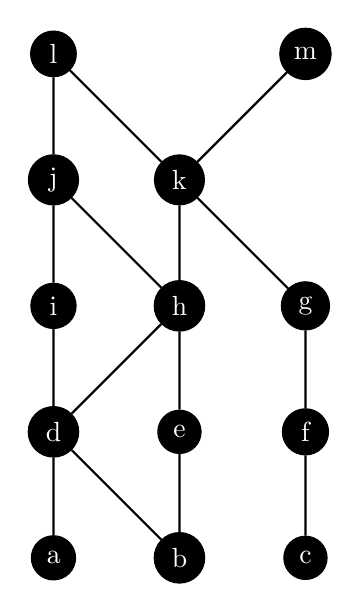
\begin{tikzpicture}[scale=0.8]
      \tikzstyle{node} = [draw,circle,fill=black,text=white]

      \def\nodes{a,b,c,d,e,f,i,h,g,j,k}
      \foreach \n/\p
      [count=\i from 0,
      evaluate= \i as \x using {2*Mod(\i,3)},
      evaluate= \i as \y using {2*int(\i/3)}]
      in \nodes {
        \node[node](\n) at (\x,\y) {\n};
      }
      \node[node](l) at (0,8) {l};
      \node[node](m) at (4,8) {m};

      \draw[thick,-] (a) -- (d) -- (i) -- (j) -- (h) -- (d) -- (b) -- (e) -- (h) -- (k) -- (l) -- (j);
      \draw[thick,-] (c) -- (f) -- (g) -- (k) -- (m);
      
    \end{tikzpicture}
  \end{minipage}
  \begin{minipage}{.65\textwidth}
    \begin{parts}
    \part[2] Find the maximal elements.
    \part[2] Find the minimal elements.
    \part[1] Is there a greatest element? If so, what is it?
    \part[1] Is there a least element? If so, what is it?
    \part[2] Find all upper bounds of $\{a,b,c\}$.
    \part[1] Find the least upper bound of $\{a,b,c\}$, if it exists.
    \part[2] Find all lower bounds of $\{f,g,h\}$.
    \part[1] Find the greatest lower bound of $\{f,g,h\}$, if it exists.
    \end{parts}
  \end{minipage}
  \begin{solution}
    % Write your solutions here
    \begin{parts}
      \part l, m
      \part a, b, c
      \part no
      \part no
      \part k, l, m
      \part k
      \part no lower bounds
      \part no lower bounds
    \end{parts}
  \end{solution}
  
\end{questions}

\end{document}

%%% Local Variables:
%%% mode: latex
%%% TeX-master: t
%%% End:
